\section{History of Online Social Networks}
\begin{figure}[h!]
\begin{center}
  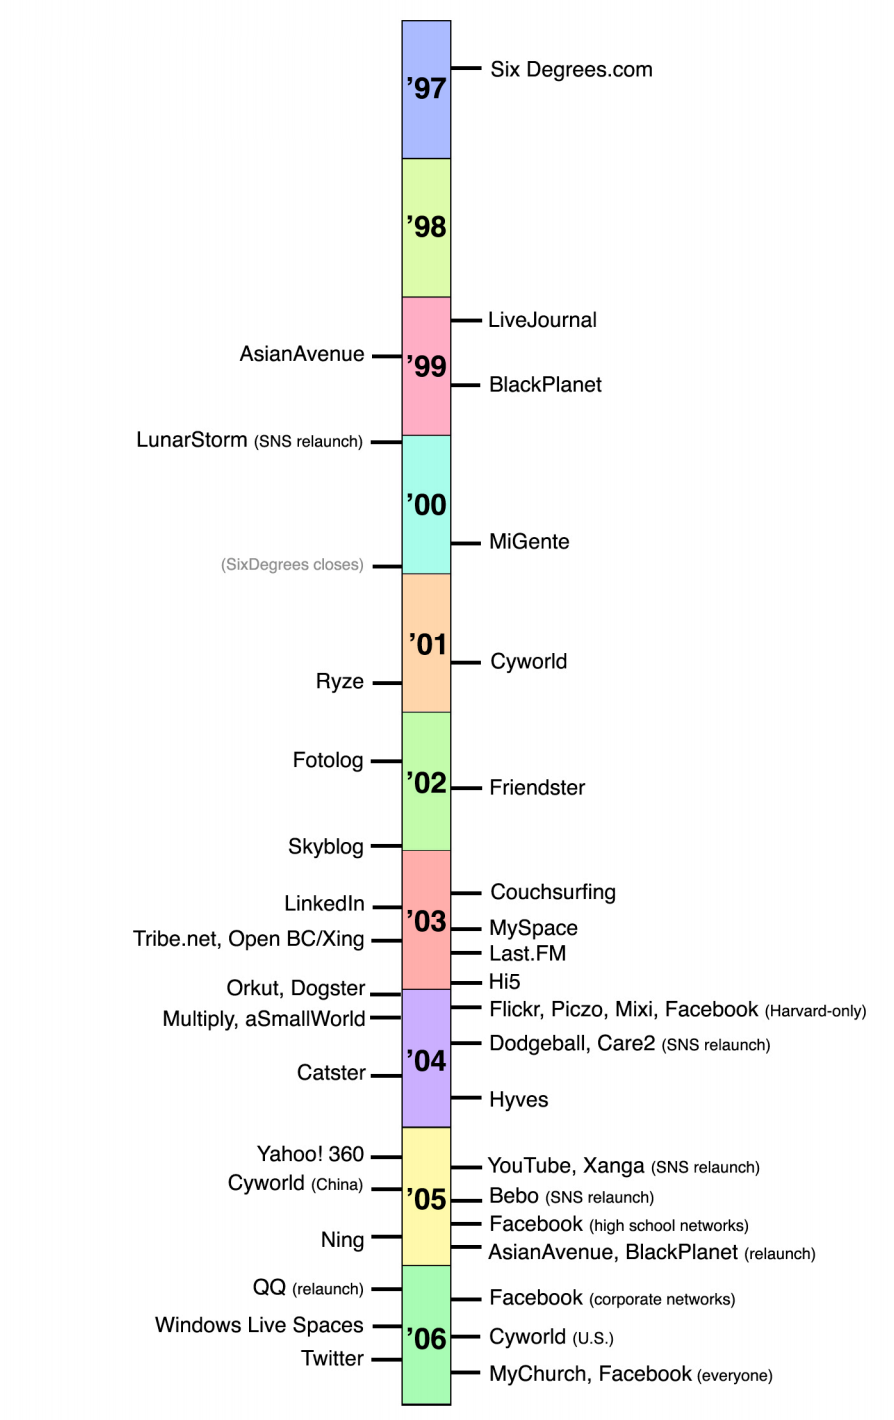
\includegraphics[width=0.7\textwidth]{img/timeline.png}
\end{center}
\caption{\label{img:timeline} Launch dates of major \glspl{osn}. (\cite{ellison2007social})}
\end{figure}

Although the first platform possessing some of the main characteristics that define \glspl{osn},
according to \cite{ellison2007social}, the first recognizable \gls{osn} launched in 1997 as we can observe in the Figure \ref{img:timeline}. \textit{SixDegrees.com} allowed users to create personal
profiles, connect with friends and consult friends of friends lists. The profile feature came from the
online dating sites and online communities, while the surfing through register users in the network
and consulting friends was an existing feature in Classmates.com. \textit{SixDegrees.com} was the first to combine
these features.

\textit{SixDegrees} promoted itself as a tool to help people to connect, but in 2000, it became an
unsustainable business and the service closed. At the time the creators conclude that
\textit{SixDegrees} was a service that was very ahead of its time.

Until 2002 many \glspl{osn} have emerged, but still incapable of projecting themselves at a global scale.
As we can observe in the timeline of Figure \ref{img:timeline} from 2002 and 2005 the \textit{big players} came to existence, in these period, \gls{osn}
such as Friendster, LinkedIn, MySpace, Hi5, Facebook and Youtube were born, shaping the business, cultural
and research landscape.
